% This Latex poster uses the baposter class, originally from
% http://www.brian-amberg.de/uni/poster. Versions are found in several places.
% The files on which this version is based are from circulation within WASP
% and exact origins are not known.
%
% CONTENT
% To update the poster, modify the contents in the parts/ folder.
% The file header.tex contains convenience commands such as \title, \companylogo etc.
% Other files contain pure formatting.
%
% COLORS
% The following standard colors are defined: wasp_text, wasppink, waspgrey, waspblue
%
% Enjoy!
% Per Skarin, 2021

\documentclass[a0paper,portrait]{baposter}
\usepackage{lipsum}  
\usepackage{relsize}	% For \smaller
\usepackage{url}	% For \url
\usepackage{epstopdf}	% Included EPS files automatically converted to PDF to include with pdflatex
\usepackage[utf8]{inputenc} 
\usepackage{multirow}
\usepackage{booktabs}
\usepackage[labelfont=bf]{caption}
\usepackage{enumitem}
\usepackage{tcolorbox}
\usepackage{mathtools}

% PATHS
\graphicspath{{template-images/}{content-images/}}

% FONTS AND COLORS
\renewcommand{\familydefault}{\sfdefault}
\newcommand{\mytitlefont}{\fontfamily{\familydefault}\selectfont }
\newcommand{\mytextfont}{\fontfamily{\familydefault}\selectfont }
% Comment the four lines below to skip WASP fonts
% \usepackage{MinionPro}
% \usepackage{MyriadPro}
% \renewcommand{\mytitlefont}{\fontfamily{MyriadPro-LF}\selectfont }
% \renewcommand{\mytextfont}{\fontfamily{MinionPro-LF}\selectfont }

\definecolor{wasppink}{RGB}{203,166,169} 
\definecolor{waspgrey}{RGB}{88,89,91}
\definecolor{waspblue}{RGB}{26,141,173}
\definecolor{darkgreen}{rgb}{0,0.6,0}

\definecolor{wasp_text}{RGB}{66,80,82}
\colorlet{wasp_banner_light}{waspblue}
\colorlet{wasp_banner_dark}{waspgrey}

% LIST SETTINGS
\setlist{itemsep=.1em, leftmargin=1em}

% COMMANDS
\newcommand\thetitle{}\renewcommand\title[1]{\renewcommand\thetitle{#1}}
\newcommand\theauthor{}\renewcommand\author[1]{\renewcommand\theauthor{#1}}
\newcommand\thedepinfo{}\newcommand\depinfo[1]{\renewcommand\thedepinfo{#1}}
\newcommand\thesupervisors{}\newcommand\supervisors[1]{\renewcommand\thesupervisors{#1}}
\newcommand\theuniversitylogo{}\newcommand\universitylogo[1]{\renewcommand\theuniversitylogo{#1}}
\newcommand\thecompanylogo{}\newcommand\companylogo[1]{\renewcommand\thecompanylogo{#1}}


%%%%%%%%%%%%%%%%%%%%%%%%%%%%%%%%%%%%%%%%%%%%%%%%%%%%%%%%%%%%%%%%%%%%%%%%%%%%%%%
%%% Document Start %%%%%%%%%%%%%%%%%%%%%%%%%%%%%%%%%%%%%%%%%%%%%%%%%%%%%%%%%%%%
%%%%%%%%%%%%%%%%%%%%%%%%%%%%%%%%%%%%%%%%%%%%%%%%%%%%%%%%%%%%%%%%%%%%%%%%%%%%%%%

% Text to the left
\title{Probabilistic and robust speech synthesis}
\author{Shivam Mehta, KTH Royal Institute of Technology}
\depinfo{Department of Speech, Music and Hearing}
\supervisors{Gustav Eje Henter (KTH) and Jonas Beskow (KTH)}

% Logos on the right. Put the images in template-images/
\universitylogo{\includegraphics[width=0.3\textwidth]{university/kth}}
% \companylogo{\includegraphics[width=0.6\textwidth]{company/ericsson}}



\begin{document}

%%% General Poster Settings %%%%%%%%%%%%%%%%%%%%%%%%%%%%%%%%%%%%%%%%%%%%%%%%%%%
%%%%%% Eye Catcher, Title, Authors and University Images %%%%%%%%%%%%%%%%%%%%%%
\begin{poster}{
 % Show grid to help with alignment
 grid=false,
 % eyecatcher=false,
 % Column spacing
 colspacing=1em,
 columns=2,
 boxpadding=.5cm,
 % Color style
 headerColorOne=wasp_banner_light,
 borderColor=wasp_banner_light,
 headerFontColor=cyan!10!white,
 % Format of textbox
 textborder=faded,
 % Format of text header
 headerborder=open,
 headershape=roundedright,
 headershade=plain,
 background=none,
 % bgColorOne=cyan!10!white,
 headerheight=0.12\textheight}
%%% Eye Cacther %%%%%%%%%%%%%%%%%%%%%%%%%%%%%%%%%%%%%%%%%%%%%%%%%%%%%%%%%%%%%%%
{
	Eye Catcher, empty if option eyecatcher=false - unused
}
%%%% Title %%%%%%%%%%%%%%%%%%%%%%%%%%%%%%%%%%%%%%%%%%%%%%%%%%%%%%%%%%%%%%%%%%%%%
{
	\textcolor{wasp_text}{\mytitlefont \huge \thetitle}
}
%%% Authors %%%%%%%%%%%%%%%%%%%%%%%%%%%%%%%%%%%%%%%%%%%%%%%%%%%%%%%%%%%%%%%%%%%
{
  \vspace{0.5em}
  \textcolor{wasp_text}{\Large \theauthor\\
	\large \thedepinfo\\
	Supervisors: \thesupervisors\\
	}
}
%%% Logo %%%%%%%%%%%%%%%%%%%%%%%%%%%%%%%%%%%%%%%%%%%%%%%%%%%%%%%%%%%%%%%%%%%%%%
{
  \begin{minipage}{8cm}
   \centering
   \vspace{0.5cm}
	    \theuniversitylogo\vspace{0.25cm}\par
		  \thecompanylogo
  \end{minipage}
}

%%%%%%%%%%%%%%%%%%%%%%%%%%%%%%%%%%%%%%%%%%%%%%%%%%%%%%%%%%%%%%%%%%%%%%%%%%%%%%
%%% Now define the boxes that make up the poster
%%%---------------------------------------------------------------------------
%%% Each box has a name and can be placed absolutely or relatively.
%%% The only inconvenience is that you can only specify a relative position 
%%% towards an already declared box. So if you have a box attached to the 
%%% bottom, one to the top and a third one which should be inbetween, you 
%%% have to specify the top and bottom boxes before you specify the middle 
%%% box.
%%%%%%%%%%%%%%%%%%%%%%%%%%%%%%%%%%%%%%%%%%%%%%%%%%%%%%%%%%%%%%%%%%%%%%%%%%%%%%

%%%%%%%%%%%%%%%%%%%%%%%%%%%%%%%%%%%%%%%%%%%%%%%%%%%%%%%%%%%%%%%%%%%%%%%%%%%%%%
  \headerbox{\mytitlefont Motivation \& Research Goals}{name=description,column=0,row=0,span=2}{
  \mytextfont
%%%%%%%%%%%%%%%%%%%%%%%%%%%%%%%%%%%%%%%%%%%%%%%%%%%%%%%%%%%%%%%%%%%%%%%%%%%%%%
  % Put the motivation behind and goals of the research here
\large
% \lipsum[2]
Natural speech is varied in nature and differs from person to person. Every individual has a different way of speaking the same text. Regressing towards the mean results in flat and dull prosody resulting in unnatural sounding synthesis. To solve this issue we need probabilistic synthesis that can define a distribution over spoken utterances thus, generating more lively speech. Moreover, aligning text and speech is a challenging problem in TTS systems which is currently dominated by attention. But attention in neural TTS systems is not monotonic, it is slow to train, it can break down into gibberish, and it requires a substantial amount of data to work. Different methods have been proposed\textsuperscript{[1, 3]} to replace attention in neural TTS systems with HMMs. We investigate the use of neural HMMs to align the text and speech more robustly \textsuperscript{[2]}
 to get the best of both words. Further, we use normalising flows to learn a distribution over the spoken utterances and sample probabilistically.
}

%%%%%%%%%%%%%%%%%%%%%%%%%%%%%%%%%%%%%%%%%%%%%%%%%%%%%%%%%%%%%%%%%%%%%%%%%%%%%%
  \headerbox{\mytitlefont Methods}{name=motivation,column=0,row=0,span=1, below=description}{
%%%%%%%%%%%%%%%%%%%%%%%%%%%%%%%%%%%%%%%%%%%%%%%%%%%%%%%%%%%%%%%%%%%%%%%%%%%%%%
  \mytextfont
  % The methods that you use goes here
We combine left-to-right HMMs defined by neural networks with normalising flows to learn the distribution over the spoken utterances conditioned on text.
\vspace{0.3cm}
\begin{center}
  \vspace{-0.4cm}
  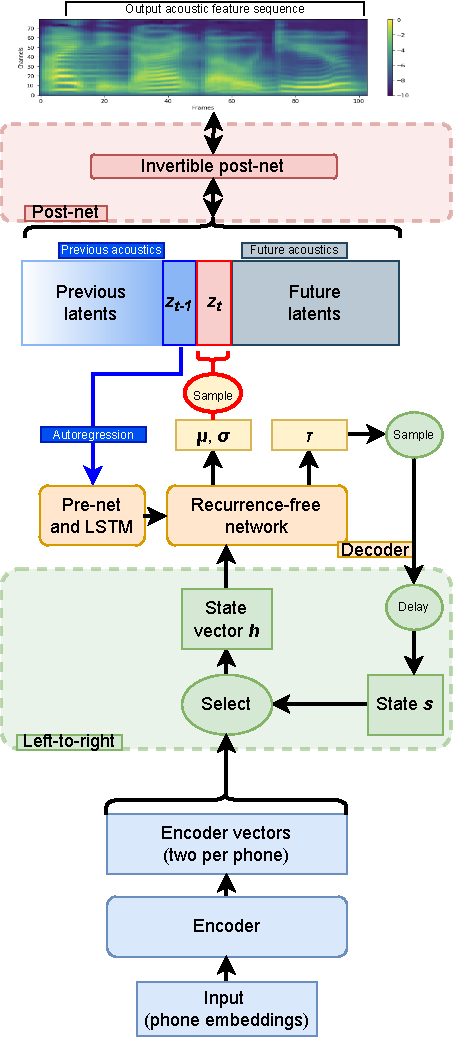
\includegraphics[height=\linewidth]{OverFlow.pdf}  
  \vspace{-0.4cm}
\end{center}
\vspace{0.25em}

Neural HMMs describe a distribution over discrete-time sequences, typically %(but not necessarily) 
assuming a Gaussian distribution for each frame.
Normalising flows,
provide a method for turning simple \emph{latent} or \emph{source} distributions $Z$, such as Gaussians, into much more flexible \emph{target} distributions $X$ through deep learning.  
The idea is to apply an invertible nonlinear transformation $f$ to the source distribution to obtain the target distribution, as $X=f(Z;\,W)$, where $f$ is parameterised by a neural network with weights $W$ and 
%To ensure invertibility we require that 
$x$ and $z$ have the same dimensionality.
%The main advantage of 
Invertibility allows us to compute the (log-)probability of %any observed outcome 
$x$ using the change of variables formula
\begin{align*}
\ln p_{X}(x)
& = \ln p_{Z}(f^{-1}(x;\,W))
+ \ln \vert \det J_{f^{-1}}(x;\,W) \vert
\text{,}
\end{align*}
where $J_{f^{-1}}(x;\,W)$ is the Jacobian matrix of $f^{-1}$ evaluated at $x$.
% \vspace{1em} % Fill in to put references at the bottom

}

%%%%%%%%%%%%%%%%%%%%%%%%%%%%%%%%%%%%%%%%%%%%%%%%%%%%%%%%%%%%%%%%%%%%%%%%%%%%%%
  \headerbox{\mytitlefont Results}{name=goal,column=1,row=1,span=1, below=description }{
%%%%%%%%%%%%%%%%%%%%%%%%%%%%%%%%%%%%%%%%%%%%%%%%%%%%%%%%%%%%%%%%%%%%%%%%%%%%%%
  \mytextfont
  % Put some results here

\begin{tcolorbox}
    \begin{center}
        Intelligibility during training
    \end{center}	

\end{tcolorbox}
	 	 %\textsuperscript{[2]}test\par
\begin{center}
	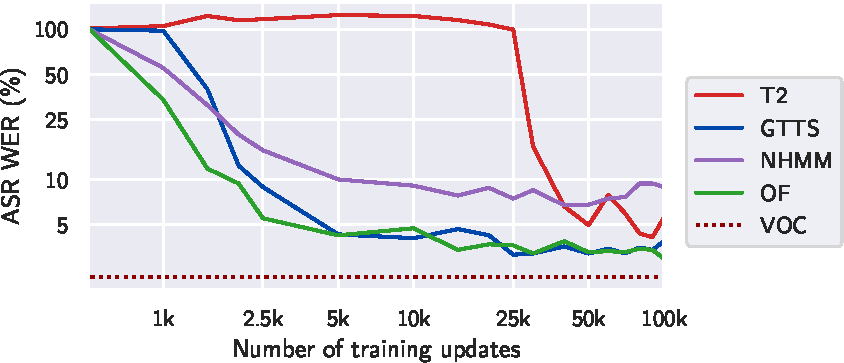
\includegraphics[width=.9\linewidth]{asr_wer.pdf}
\end{center}
Here, we plot the Word Error Rate (WER) of the synthesised utterances using the test set's synthesised utterances during the course of training. We plot our proposed system OverFlow (OF) with baseline methods namely, Tacotron 2 (T2), Glow-TTS (GTTS), Neural-HMM\textsuperscript{[3]}, along with the vocoded speech (VOC). Our model converges faster to a lower WER than all the other baselines.

\vspace{1.5em}

\begin{tcolorbox}
    \begin{center}
        Subjective listening test
    \end{center}
\end{tcolorbox}

\begin{center}
	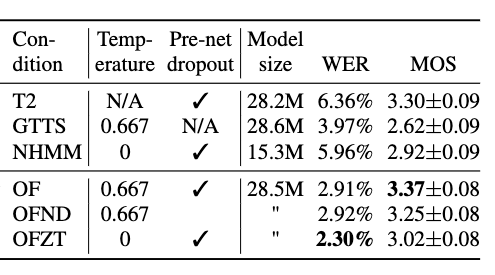
\includegraphics[width=.9\linewidth]{results_table.png}
\end{center}
In a subjective listening test, our method (OF) performs the best compared to other systems while being statistically comparable to T2. Other OF conditions, OFND: OverFlow with No Dropout in prenet and OFZT: OverFlow with Zero Temperature perform fairly in the listening test. Further, we resynthesised the 720 Harvard sentences [32], which are ideal for evaluating intelligibility since they are phonetically balanced. All OverFlow conditions perform substantially better than all baselines on these simple out-of-domain sentences.
\par
\vspace{1.5em}
\par
% \begin{tikzpicture}
% 	\node[anchor=west] at (0,0) {
% 		\begin{minipage}{0.2\textwidth}
% 		\centering
% 		\resizebox{\textwidth}{!}{\includegraphics{homer_smart}}
% 		\end{minipage}
% 	};
% 	\node[anchor=east] at (\textwidth,0) {
% 		\begin{minipage}{0.7\textwidth}
% 		\begin{tcolorbox}
% Test \textsuperscript{[3]}.
% 		\end{tcolorbox}
% 		\end{minipage}
% 	};
% \end{tikzpicture}
% \vspace{1.5em}
% \begin{tcolorbox}
% 	test4
% \end{tcolorbox}


}
%%%%%%%%%%%%%%%%%%%%%%%%%%%%%%%%%%%%%%%%%%%%%%%%%%%%%%%%%%%%%%%%%%%%%%%%%%%%%%
  \headerbox{\mytitlefont Results}{name=goal,column=1,row=2,span=1, below=description }{
%%%%%%%%%%%%%%%%%%%%%%%%%%%%%%%%%%%%%%%%%%%%%%%%%%%%%%%%%%%%%%%%%%%%%%%%%%%%%%
  \mytextfont
  % Put some results here

\begin{tcolorbox}
    \begin{center}
        Intelligibility during training
    \end{center}	

\end{tcolorbox}
	 	 %\textsuperscript{[2]}test\par
\begin{center}
	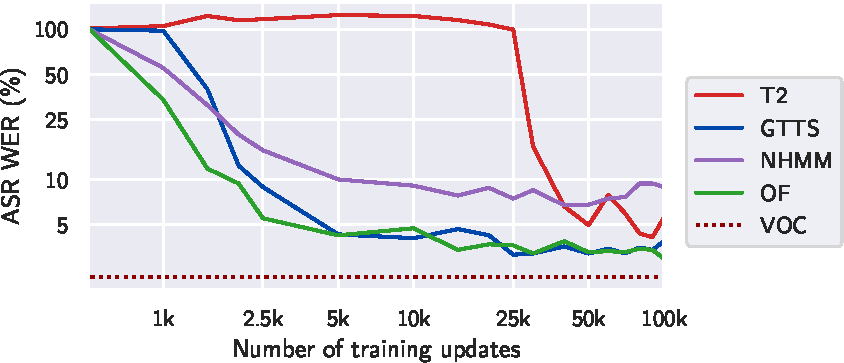
\includegraphics[width=.9\linewidth]{asr_wer.pdf}
\end{center}
Here, we plot the Word Error Rate (WER) of the synthesised utterances using the test set's synthesised utterances during the course of training. We plot our proposed system OverFlow (OF) with baseline methods namely, Tacotron 2 (T2), Glow-TTS (GTTS), Neural-HMM\textsuperscript{[3]}, along with the vocoded speech (VOC). Our model converges faster to a lower WER than all the other baselines.

\vspace{1.5em}

\begin{tcolorbox}
    \begin{center}
        Subjective listening test
    \end{center}
\end{tcolorbox}

\begin{center}
	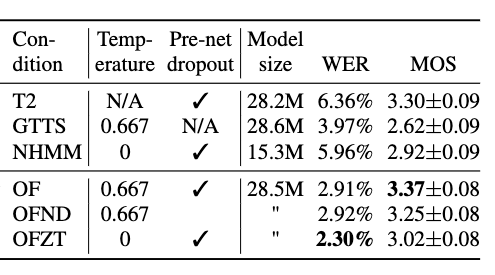
\includegraphics[width=.9\linewidth]{results_table.png}
\end{center}
In a subjective listening test, our method (OF) performs the best compared to other systems while being statistically comparable to T2. Other OF conditions, OFND: OverFlow with No Dropout in prenet and OFZT: OverFlow with Zero Temperature perform fairly in the listening test. Further, we resynthesised the 720 Harvard sentences [32], which are ideal for evaluating intelligibility since they are phonetically balanced. All OverFlow conditions perform substantially better than all baselines on these simple out-of-domain sentences.
\par
\vspace{1.5em}
\par
% \begin{tikzpicture}
% 	\node[anchor=west] at (0,0) {
% 		\begin{minipage}{0.2\textwidth}
% 		\centering
% 		\resizebox{\textwidth}{!}{\includegraphics{homer_smart}}
% 		\end{minipage}
% 	};
% 	\node[anchor=east] at (\textwidth,0) {
% 		\begin{minipage}{0.7\textwidth}
% 		\begin{tcolorbox}
% Test \textsuperscript{[3]}.
% 		\end{tcolorbox}
% 		\end{minipage}
% 	};
% \end{tikzpicture}
% \vspace{1.5em}
% \begin{tcolorbox}
% 	test4
% \end{tcolorbox}


}

%%%%%%%%%%%%%%%%%%%%%%%%%%%%%%%%%%%%%%%%%%%%%%%%%%%%%%%%%%%%%%%%%%%%%%%%%%%%%%
  \headerbox{References}{headerColorOne=wasp_banner_dark, borderColor=wasp_banner_dark, name=results,column=0,row=0,span=1, below=motivation }{
%%%%%%%%%%%%%%%%%%%%%%%%%%%%%%%%%%%%%%%%%%%%%%%%%%%%%%%%%%%%%%%%%%%%%%%%%%%%%%
	\mytextfont
  \small
% \vspace{-0.5cm}
% \fcolorbox{white}{white}{\hspace{-0.5cm}\parbox{0.1\linewidth}{\centering [1]}\parbox{1.3cm}{\includegraphics[trim=28mm 10mm 35mm 15mm,clip,width=0.8cm]{qracm}}\parbox{0.7\linewidth}{\footnotesize\smaller Five Challenges in Cloud-Enabled Intelligence and Control\\\tiny T. Abdelzaher, Y. Hao, K. Jayarajah, A. Misra, S. Yao, P. Skarin, D. Weerakoon and K. {\AA}rz{\'e}n\\ACM Transactions on Internet Technology, 2019}}\par\vspace{-0.4cm}

\vspace{-0.5cm}
\fcolorbox{white}{white}{\hspace{-0.5cm}\parbox{0.1\linewidth}{\centering [1]}\parbox{0.9\linewidth}{\footnotesize\tiny T. Fujimoto, K. Hashimoto, Y. Nankaku, and K. Tokuda, “Autoregressive variational autoencoder with a hidden semi-Markov model-based structured attention for speech synthesis,” in Proc. ICASSP, 2022.}}\par

\fcolorbox{white}{white}{\hspace{-0.5cm}\parbox{0.1\linewidth}{\centering [2]}\parbox{0.9\linewidth}{\footnotesize \tiny O. Watts, G. E. Henter, J. Fong, and C. Valentini-Botinhao, “Where do the improvements come from in sequence-to-sequence neural TTS?,” in Proc. SSW, 2019.}}\par
	
\fcolorbox{white}{white}{\hspace{-0.5cm}\parbox{0.1\linewidth}{\centering [3]}\parbox{0.9\linewidth}{\footnotesize\tiny S. Mehta, É. Székely, J. Beskow, G. E. Henter, "Neural HMMs are all you need (for high-quality attention-free TTS)", in Proc. ICASSP2022}}\par
}

\headerbox{}{name=foottext, column=0, span=2, above=bottom, textborder=none,headerborder=none,boxheaderheight=0pt,boxColorOne=wasp_banner_dark}{\hfill \includegraphics[height=1cm]{waspwhite}}


\end{poster}
\end{document}
